% ------------- DEFINITION DU DOCUMENT -------------

\documentclass[12pt, oneside]{report}
% Types de documents possibles : book, article, report, slides
% Options pour la police du document et sa mise en page globale. Se référer au manuel pour liste exhaustive.


% ------------- GESTION DES LANGUES -------------

\usepackage[english]{babel}
\usepackage[T1]{fontenc} % Ne pas utiliser si XeTeX ou LuaTeX
\usepackage[utf8]{inputenc} % Ne pas utiliser si XeTeX ou LuaTeX

% ------------- MISE EN PAGE GLOBALE -------------

% Package gérant la taille des marges. Pour plus de détails sur la mise en page, utiliser \layout
\usepackage[top=2.7cm, bottom=2.7cm, left=2.5cm, right=2.5cm]{geometry}

% Gestion des entêtes/pieds (plain : pieds, headings : en-tête, empty : rien; appliquer sur une page, \thispagestyle{})
\pagestyle{plain}
% Gestion du pack de police utilisé pour le document
\usepackage{lmodern}

%¨Police Personnalisée /!\ A Utiliser avec le moteur XeTex ou LuaTex
%\usepackage{fontspec} 
%\setmainfont{Vinci_Serif_Regular.otf}[
%BoldFont = Vinci_Serif_Bold.otf ,
%ItalicFont = Vinci_Serif_Italic.otf ,
%BoldItalicFont = Vinci_Serif_Bold_Italic.otf ]

% Mise des \todo{}
\usepackage[colorinlistoftodos]{todonotes}


% A décommenter pour ne plus afficher le header des chapitres
%\usepackage{titlesec}
%\titleformat{\chapter}
%  {\Large\bfseries} % format
%  {}                % label
%  {0pt}             % sep
%  {\huge}           % before-code


% ------------- PACKAGE DE MISE EN PAGE -------------

% Package pour la gestion des interlignes (déclaration de type environnement; onehalfspace, doublespace...)
\usepackage{setspace}
% Pour \st (barrer) et \ul (souligner)
\usepackage{soul}
% Pour colorier le texte
\usepackage{color}
% Pour la mise en page de code source
\usepackage{listings}
% Pour les indices (\textsubscript{})
\usepackage{subscript}
% Pour utiliser les liens : \url{ } 
\usepackage{hyperref}

\usepackage{subfig}


% ------------- PACKAGE MATH -------------

% Pour ouvrir l'environnement math : $, $$, \begin{math}, et \begin{equation}

\usepackage{amsmath}
\usepackage{amssymb}
\usepackage{mathrsfs}


% ------------- INSERTION IMAGES -------------

\usepackage{graphicx}

% Inclure les images avec \includegraphics{chemin}
% Options : height=, width= ou scale=, angle=

% Environnements flottants : \begin{figure}[placement] à coupler avec une environnement d'alignement
% Options de placement : t (top), h (ici), b (bas), ...

% légendes : \caption{} à placer à la suite de l'environnement center, dans l'environnement flottant

% \clearpage crée une nouvelle page avec mise en place préalable des flottants


% ------------- TABLEAUX -------------

% Créer un tableau avec \begin{tabular}{cc} avec en 2ème accolade les alignements et le nombre de colonnes
% Options d'alignement : c, r et l, et p[largeur]
% Séparateurs : | et @{<separateur>} permettent de spécifier la position des séparateurs verticaux (a placer dans la 2ème accolade). \hline crée une ligne horizontale 

% & permet de séparer les cellules sur la même ligne. \\ crée une nouvelle ligne.

% Pour utiliser \backslashbox{}{}
\usepackage{diagbox}

% Pour créer une table : \begin{table}. Se comporte comme un flottant.


% ------------- GESTION DU CODE SOURCE ET ALGO -------------

\lstset{
language=C++,        		% choix du langage (C, C++, Java, PHP, SQL, XML, HTML, ...). Peut se choisir localement avec language=
basicstyle=\footnotesize,       % taille de la police du code
numbers=left,                   % placer le numéro de chaque ligne à gauche (left)
numberstyle=\normalsize,        % taille de la police des numéros
numbersep=10pt,                  % distance entre le code et sa numérotation
backgroundcolor=\color{white},  % couleur du fond 
}
% S'utilise avec l'environnement \begin{lstlisting}[frame=one] et \lstinputlisting{fichier_source}

\usepackage[linesnumbered]{algorithm2e}


% ------------- TITRE -------------

% Création de la page de titre avec \maketitle


% ------------- TABLE DES MATIERES -------------

% Création de la table des matières avec \tableofcontents

% Redéfinit le titre de la table des matières
\AtBeginDocument{\renewcommand{\contentsname}{Table des Matières}}
% Indique les éléments à inclure : -1 correspond aux parties, 5 aux sous-paragraphes
\setcounter{tocdepth}{3}


% ------------- CORPS DU DOCUMENT -------------

\begin{document}

\begin{center}
\Large{
\textbf{DH2323 Project Report : \\ Implementing a basic pathtracer}
} 
\medskip
\small{\\Jonathan Guichard (jgui@kth.se - 941028-3577) \\ Project blog : \url{https://dh2323jgui.wordpress.com/}}
\end{center}

\bigskip

\section*{Introduction}

\paragraph{}Pathtracing is a method of rendering images of three-dimensional scenes such that the illumination is faithful to the reality. It simulates many effects "out-of-the-box", such as shoft shadows, ambient occlusion and indirect lighting, that otherwise have to be coded into other rendering methods, for example such as raytracing. The fundamental principle consists of casting light rays starting from the camera, then recursively casting new random rays in order to determine the color of the hit area. This method makes use of Monte Carlo integration and the rendering equation.

\section*{Initial specification}

\paragraph{}The goal of this project is to implement a very simple pathtracer, capable of rendering a scene of the same complexity as the one used in labs 2 and 3 of the rendering track. \\
In other words, the pathtracer we implement must be capable of rendering a simple Cornell Box with a fixed surface light source on the roof, of variable size and emitted color. The camera has a fixed position and can not rotate, and we consider all the objects present in the scene to be made of the same material and to be ideally diffuse. We do not render any complex materials and phenomenons that would require some specific handling, such as water, glass, specular surfaces or caustics, to only name a few. \\

\paragraph{}The objective of this project is to be able to render a cornell box and to compare pathtracing to the two other different rendering methods implemented during the labs of the rendering track. 

\section*{Related work}

\paragraph{}The original pathtracing algorithm was first proposed by Kajiya in \emph{The Rendering Equation} \cite{renderingEquation}, in 1986. This is the algorithm we will implement in this project.

\paragraph{}An improved version of this pathtracing algorithm was introduced by Lafortune and Willems in 1993 \cite{BDPT}. This algorithm is an improvement of pathtracing, as it significantly improves the performances for indoor scenes where indirect lighting is important, and it is also able to better deal with complex phenomenons such as light caustics. The basic principle 

\section*{Theoretical aspects}

\paragraph{}Pathtracing is quite similar to raytracing, as for each pixel, rays are traced from the camera to determine a collision point with the scene we are rendering. However, once the collision point has been determined, we do not use mathematical models to determine the illumination of this point, but rather try to simulate at a lower level what whould physically happen in reality. 

\paragraph{}The rendering equation \cite{renderingEquation} is the cornerstone of pathtracing, and tells us how we should compute outgoing light from an intersection point $x$. It is as follows (we consider that all the wave lengths have the same behavior) : 

\begin{align}
	L_{o}(w_{o}, x) = L_{e}(w_{o}, x) + \int_{\Omega} f(w_{i}, w_{o}, x) L_{i}(w_{i}, x)(w_{i} \cdot n) dw_{i}
\end{align}

\paragraph{}Where $w_{o}$ is the direction of the outgoing light, $w_{i}$ the direction of the incoming light, $f$ is the bidirectional reflectance distribution function, $n$ the normal of the surface hit by the ray, and $L$ the radiance. In other words, the light we see when looking at an object is made up of the light emitted by this object and by the reflected light in our viewing direction from light that is hitting the point $x$ on the object from all possible directions.

\paragraph{}However, in order to determine the radiance of the outgoing light, we need to compute an integral over an hemisphere centered around the normal of the surface as equation (1) shows us. In order to compute that integral, we make use of what is called Monte Carlo Integration. The idea is to randomly choose some elements in the integration domain $\Omega$, and use those elements only in order to approximate the true value of the integral. In mathematical terms, we would approximate an integral $I$ with $\widetilde{I}$ as follows \cite{scratchapixel} :

\begin{align}
	\widetilde{I} = \frac{1}{N} \sum_{i=0}^{N-1} \frac{f(X_{i})}{pdf(X_{i})}
\end{align}

\paragraph{}Where $N$ is the number of samples, $X_{i}$ a random sample belonging to the integration domain, and $pdf$ the probability distribution function for selecting a random sample. When performing a uniform sampling, which is our case, this simply becomes an average of uniformly randomly selected rays, as the probability density function is the same for every sample. The bigger the number of samples, the closer we should be to the real value.

\paragraph{}Putting those two theoretical elements together, the following pseudocode would be the "heart" of our pathtracer. It computes the outgoing light from a point $x$ situated on an object surface :

\clearpage

\begin{algorithm}[h]
$reflected\_light = 0$\;
\Repeat{$number\_of\_samples = N$}{
	Pick a random direction $\vec{d}$ at uniform probability such that $\vec{d} \cdot \vec{n} \ge 0$, with $\vec{n}$ the normal of the surface hit\;
	$cos \leftarrow \vec{d} \cdot \vec{n}$\;
	$BRDF \leftarrow 2 * reflectance\_surface * cos$\;
	$reflected\_light \leftarrow reflected\_light + incoming\_light\_from(x, \vec{d}) * BRDF$\;
}
$ outgoing\_light = emitted\_light\_by\_surface + reflected\_light / N$\;
\label{alg:basics}
\end{algorithm}

\paragraph{NB} We only handle ideally diffuse surfaces, which have the same reflectance regardless of the viewing angle, therefore we do not take this viewing angle into account in the above pseudocode.

\paragraph{} The only remaining element we need to figure out is how to know the value of the incoming light to a point and from a given direction, since we need that information when computing the reflected light. \\ The way a pathtracer handles this is through recursion : in order to know the incoming light, find the originating surface point of that light, and apply the pseudo-code presented above. We then only need to set a maximum depth limit to this recursion, in order for the program to actually be able to finish its execution. When we reach that maximum depth, we simply consider that there is no incoming light (we can see this as the light "being" perfectly black).

\paragraph{}The following figure gives a good visualization of how a pathtracer is working at its core :

\begin{figure}[h]
    \centering
    \includegraphics[width=0.3\linewidth]{pathtracing.png} 
    \caption{The base principle of pathtracing. For clarity, not all rays have been drawn. Image courtesy of www.scratchapixel.com \cite{scratchapixel}.}
    \label{fig:pathtracing}
\end{figure}

\section*{Implementation Remarks}

\paragraph{Monte Carlo Integration} In order to select a random direction within a hemisphere with a uniform probability, we chose to implement a method based on random gaussian variables, as detailed in the very last section of \cite{randomPointSphere} (equation 16). This solution is originally for picking a random point with uniform probability on a sphere, but can easily be reduced to a hemisphere. If we end up with a direction belonging to the "wrong" hemisphere, we simply invert the randomly picked vector (multiply all its elements with -1).

\paragraph{Möller-Trombore intersection algorithm} In order to speed-up the intersection computations, we decided to replace the code from Labs 2 and 3 with the Möller-Trombore intersection algorithm, which yields significantly better performances, as this method does not require matrix inversions or any other costly operations. For more details, please refer to \cite{mollerTrumbore}. \\ The thought process to solve performance issues is further detailed in the project blog.

\paragraph{Multithreading}Finally, in order to further speed up our pathtracer and take advantage of modern computing power, we decided to implement some basic multithreading. In our implementation, each pixel color is being computed in parallel, as those computations are independent and have no side effects. \\ The thought process to solve performance issues is further detailed in the project blog.

\paragraph{Gamma correction} In order to get a more faithfull rendering, we decided to implement gamma correction with $\gamma = 2.2$.

\section*{Results, Experiments and Discussions}

\paragraph{NB} The following images where generated with a depth of 3 and gamma correction of $\gamma = 2.2$, unless otherwise specified. The colors of the scene were also slightly changed on some renders to get more "popping" colors when generating them. Those color differences are therefore not caused by the rendering technique in itself, simply by a different scene definition.

\paragraph{}When running the pathtracer detailed previously, the first observation we make is that the algorithm converges quite slowly towards a noiseless image. The observed noise is directly impacted by the number of samples we choose to use. Indeed, with a low number of samples, the accuracy of the Monte Carlo estimate is lower, leading to a higher variation of the color value for neighboring pixels, which is visually expressed as noise, as shown by figure \ref{fig:noiseComparison}.

\begin{figure}[h]
    \centering
    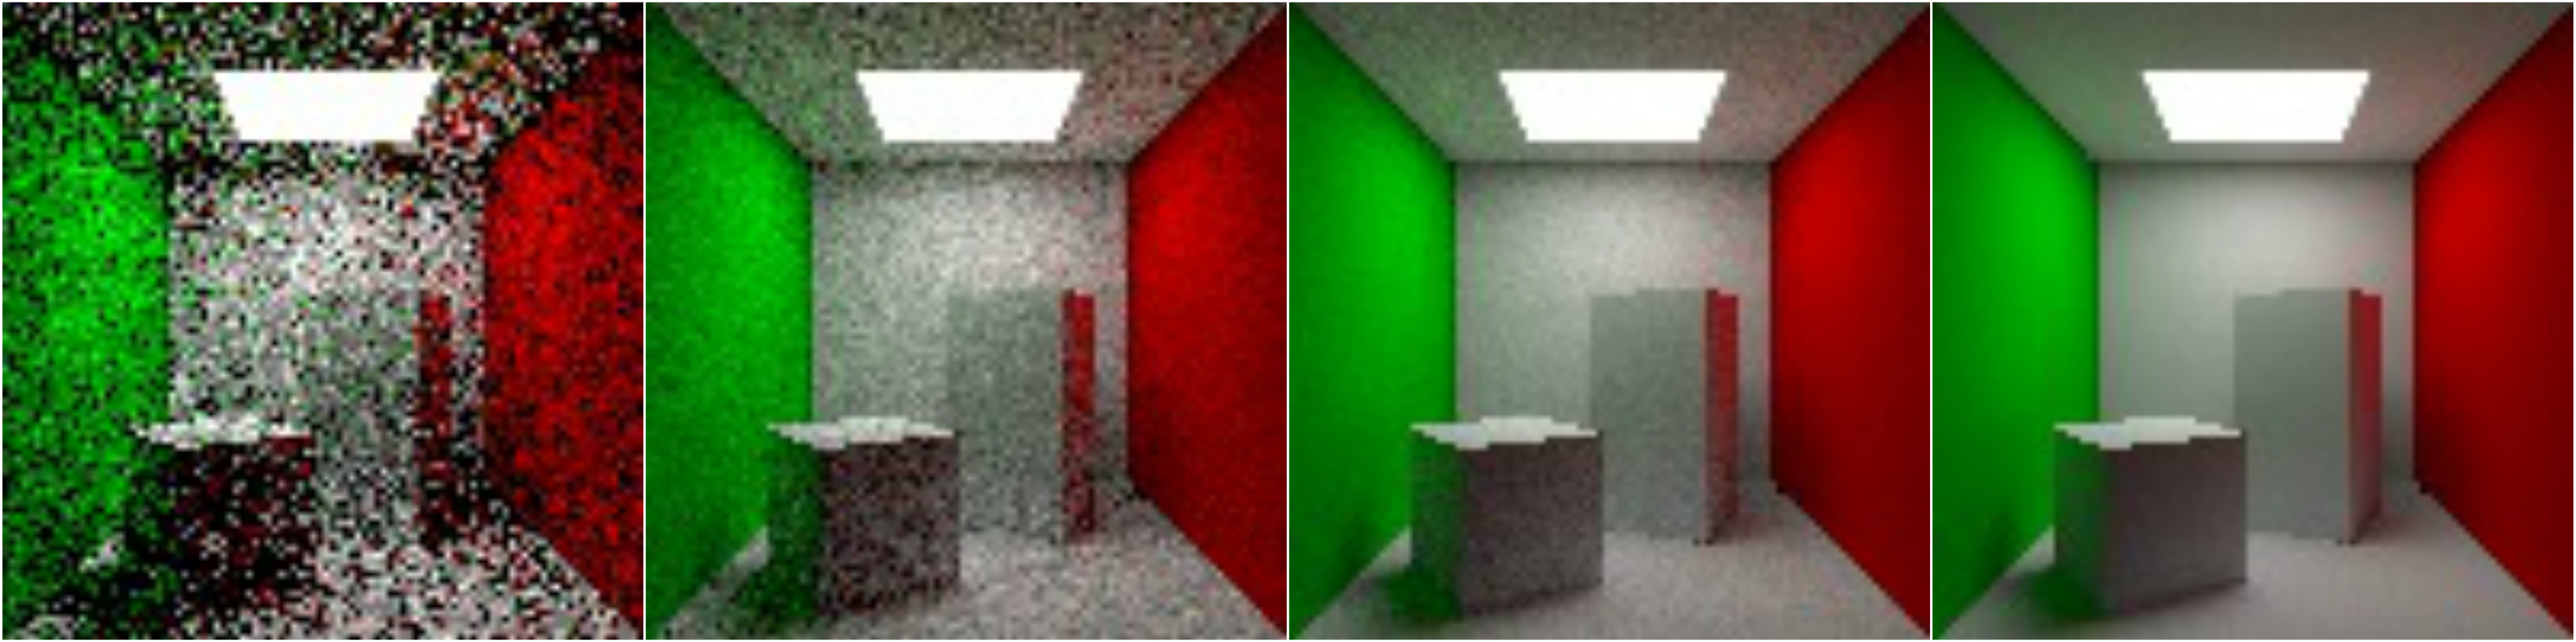
\includegraphics[width=1\linewidth]{Noise_Comparison.png} 
    \caption{Effect of the number of samples on noise in the final image. The number of samples have been multiplied by 10 for each image, going from left to right.}
    \label{fig:noiseComparison}
\end{figure}

\paragraph{}Based on this observation, we decided to slightly alter the pathtracing algorithm presented page \pageref{alg:basics}. Instead of performing a Monte Carlo integration at \emph{every} recursion step, we decide to only perform this integration at the "pixel level". We are now casting $M$ rays originating from the camera instead of just one, rays which we then average. When one of those rays hits a surface, we cast only one child ray, at uniform probability within the hemisphere centered around the normal to the surface that was hit, and so on and so forth until we reach the maximum recursion level. We of course make use of the rendering equation each time a ray hits a surface, the only difference being that we use only one sample to "perform" the Monte Carlo integration.\\
The justification behind this modification is that we want to spend more time where it really matters, that is at the pixel level. Indeed, computing a very precise light contribution at deep recursion levels will only very slightly contribute to a more accurate pixel color, if at all. We also expect any precision problems for the Monte Carlo integrations to be corrected when averaging at the pixel level. The expected result is thus less noise for a similar running time, while the image retains its original characteristics. Figure \ref{fig:fasterConv} showcases a comparison of both methods :

\begin{figure}[h]
    \centering
    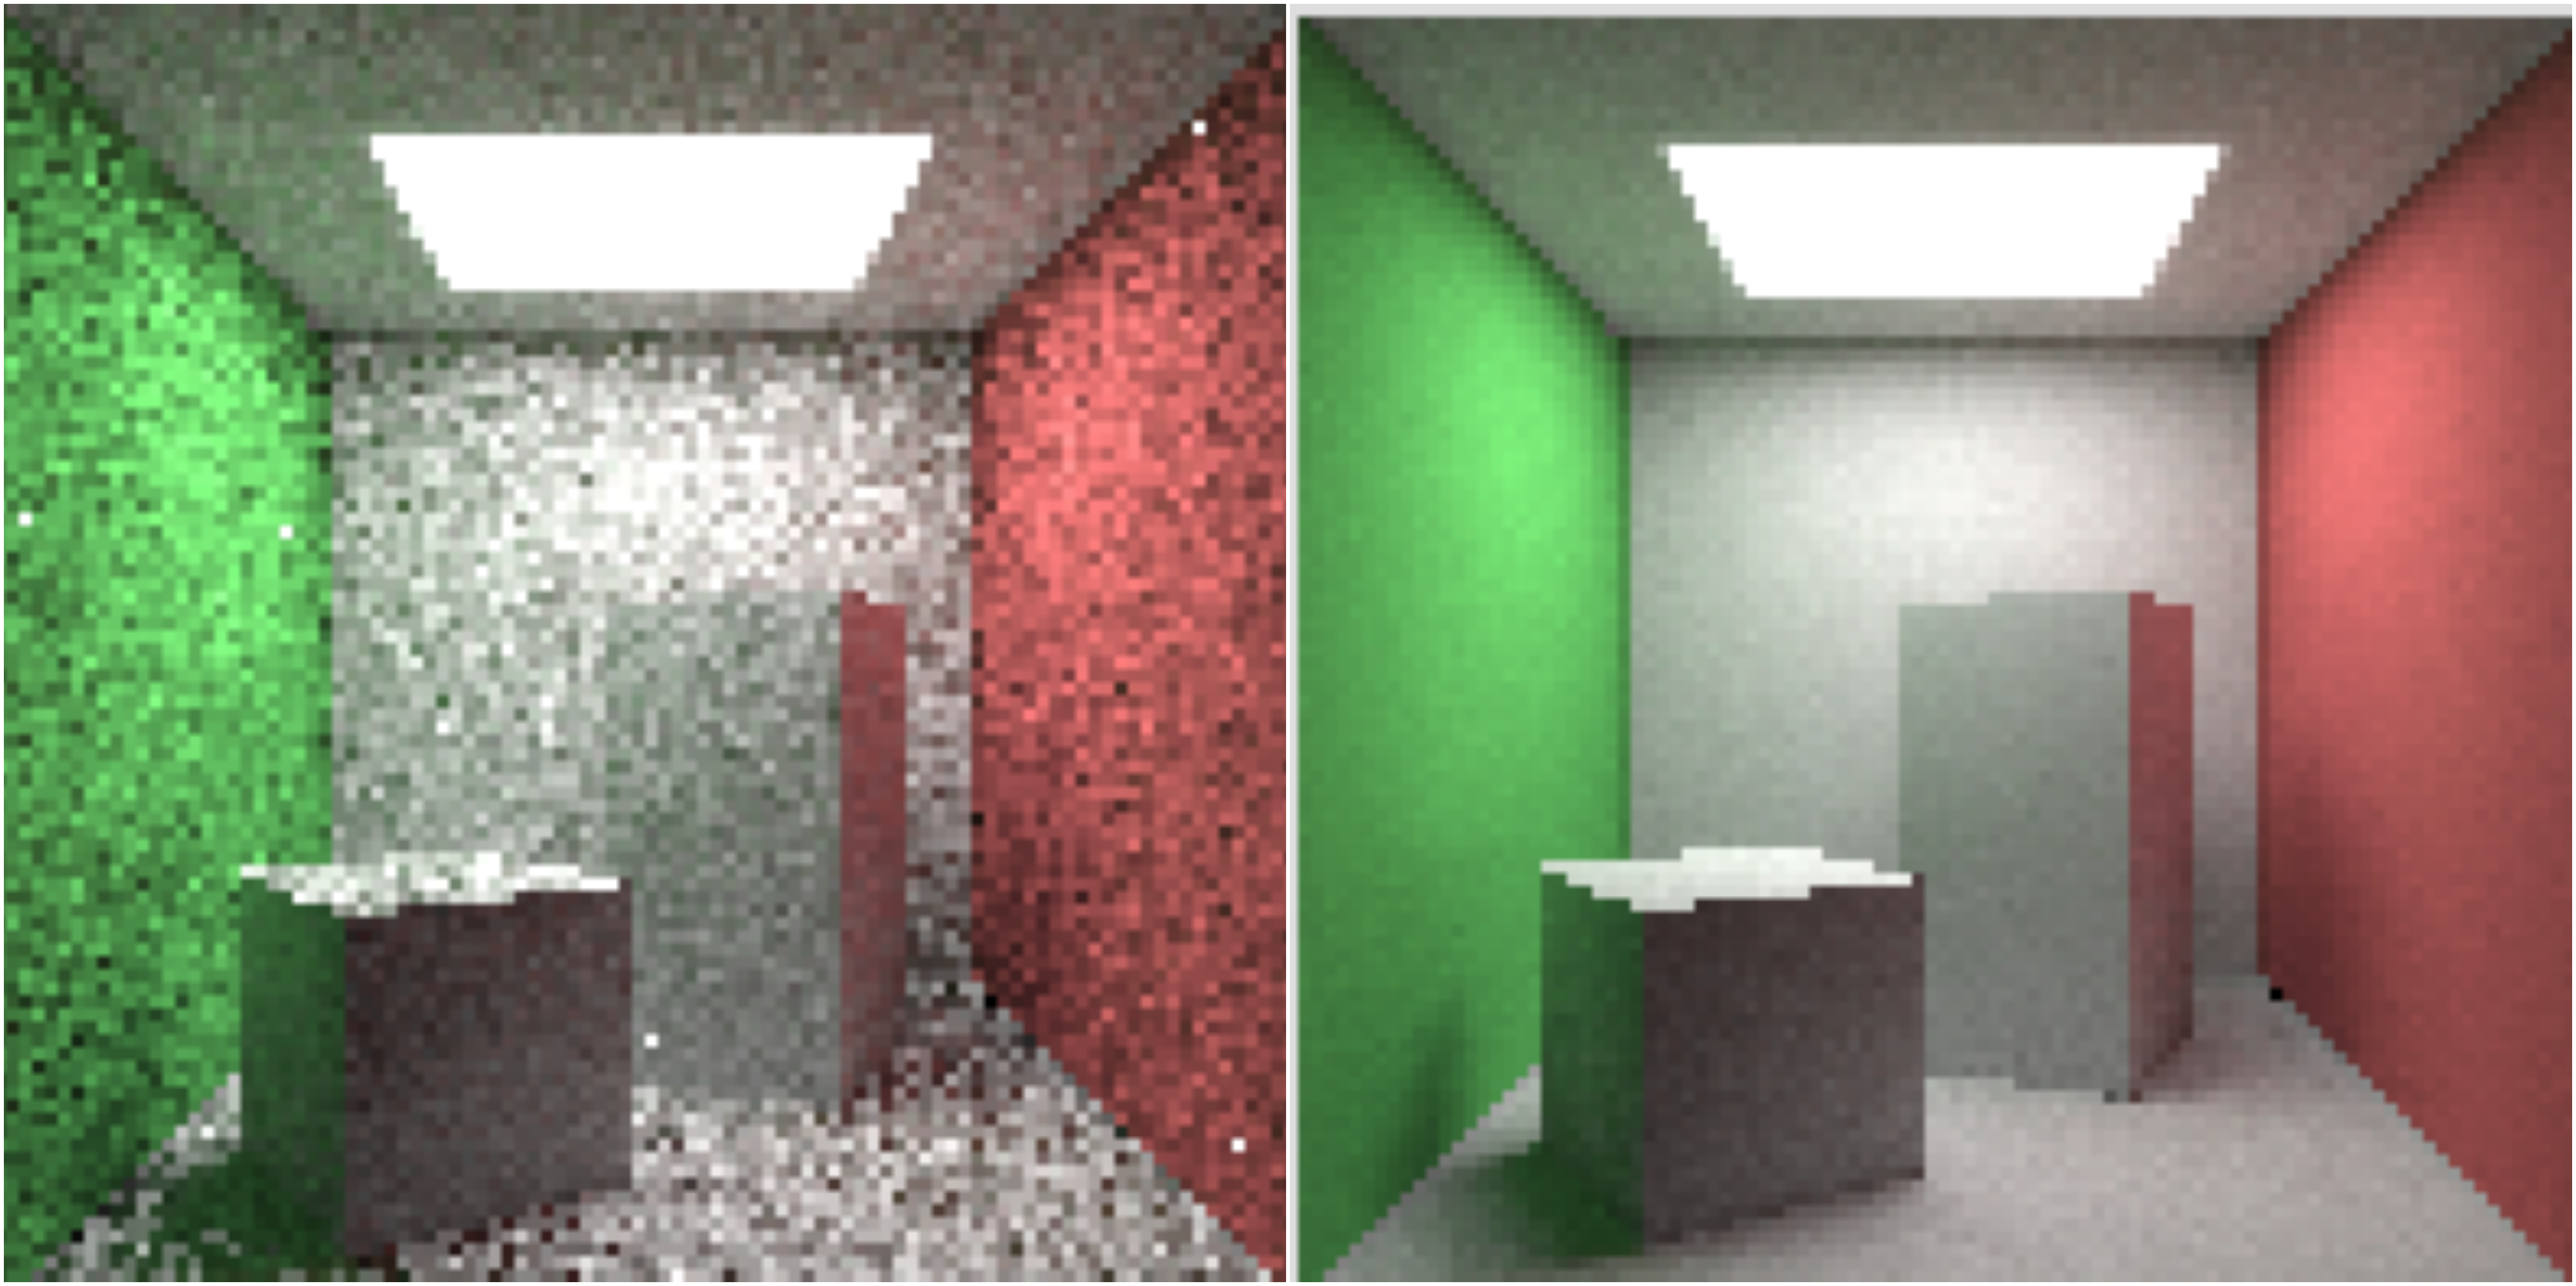
\includegraphics[width=0.6\linewidth]{faster_conv.png} 
    \caption{Comparison of the original pathtracing method (left) with the faster version (right). Those two images where generated for a similar running time.}
    \label{fig:fasterConv}
\end{figure}

\paragraph{}As we can see, there seems to be no detail loss with this new method, as we still have smooth shadows, indirect lighting, and ambient occlusion. We have therefore made the choice to keep this new method in our implementation.

\paragraph{}Figure \ref{fig:depthComparison} show us the effect of depth on the final rendered result. \\ 
When the depth is just one, we only "see" the light source and nothing else, as expected, since we are not able to compute any light component other than the emitted light. \\ 
For a depth of two, we are now able to see something else than just black and white, but the image is still not very eye-pleasing, as many areas of the picture are pitch black. Again, this can be explained by the fact that the rays don't have enough "bounces" to reach the light source, leading to some very black spots (especially for the roof, it's indeed impossible to hit the light source with just one ray starting from any point on the roof). We are still able to observe interesting features tough, such as smooth shadows and some sort of ambient occlusion.\\ 
Finally, the rendered results start to be much nicer looking for a depth of 3 or more, since we are now actually having enough bounces to eliminate the pitch black spots, and this also allows us to see some indirect lighting (we indeed need a least 3 bounces to see those features appear). Interestingly though, there is little to no visible difference when using a depth of 4 compared to a depth of 3. The contribution to the final result seems to be very minor, as one could have expected, for deeper recursion levels. A maximum recursion depth of 3 therefore seems to be the best time/details compromise.

\begin{figure}[h]
    \centering
    \includegraphics[width=1\linewidth]{depth_test.png} 
    \caption{Effect of the maximum recursion depth on the final result, varying from 1 to 4 (left to right). These images were generated with 50000 samples.}
    \label{fig:depthComparison}
\end{figure}

\paragraph{} The final result obtained for this basic pathtracer is shown in figure \ref{fig:finalResult}. The rendering time was approximately of 20 hours for 512x512 pixels on a 4-core 2.2Ghz CPU. The same scene was generated with the Raytracer from Lab 2 and the Rasterizer from Lab 3, shown in figure, for comparison. 

\begin{figure}[h]
    \centering
    \includegraphics[width=0.55\linewidth]{big_100000.png} 
    \caption{Our pathtracer rendering a Cornell box using the faster method (100000 samples per pixel).}
    \label{fig:finalResult}
\end{figure}

\paragraph{}The main conclusion we can draw from this project is that we are able to achieve very interesting and eye-pleasing results in just a few lines of code, which can be a surprising and counter-intuitive statement at first. However, some very nice features, such as indirect lighting, smooth shadows, and ambient occlusion work "out-of-the-box" for this method, while it would require some specific non-trivial handling in methods such as Raytracing or Rasterization. \\ 
As a general conclusion, we could arguee that the closer the method is to the physical reality, the less specific handling it requires and the better looking the results are, but this comes of course at the cost of performance. 

\begin{figure}[h]
    \centering
    \includegraphics[width=1\linewidth]{methods_comparison.png} 
    \caption{A similar scene being rendered by our raytracer (left, $\approx 10s$), rasterizer (center, $\approx 1s$), and pathtracer (right, $\approx 24h$).}
    \label{fig:methodsComparison}
\end{figure}

\clearpage

\section*{Discussion regarding perceptual user studies}

\bibliography{biblio}{}
\bibliographystyle{plain}


% non-implementation goals : exploring the effect of the parameters (depth and sampling) on different images, trying to explain why we see this.


\end{document}
